\documentclass[11pt]{article}
\usepackage[paper  = letterpaper,
                     left   = 1.2in,
                     right  = 1.2in,
                     top    = 1.0in,
                     bottom = 1.0in,
                     ]{geometry}

% \usepackage[bitstream-charter]{mathdesign}
\usepackage{amsmath}
\usepackage{float}
\usepackage{graphicx}



\title{C137 Project: Music Popularity Prediction}
\author{Matthew Cook, Michael Loturco, and Abigail Stone}
\date{}

\begin{document}
\maketitle

\section{Introduction}

Music streaming is a growing area with a wealth of data, access to this data gives us the opportunity to try to predict popularity and growth of songs. We assume that popularity changes over time, and thus trying to estimate ‘popularity’ without considering time dimension will produce poorer model performance than predicting popularity while considering time. 


Existing work has attempted to classify songs into buckets of popularity, ‘low’, ‘medium’ and ‘high’ or as ‘hit song’ and ‘not hit song’ by looking at extensive sets of features. Features of a track can range from lyrical(e.g. valence, mood) to metadata (e.g. artist name, album) information to actual audio features extracted from the audio file itself (e.g. danciness, energy). HitMusicNet uses a compressed and encoded set of these features as an input to a Convolutional Neural Network and outputs a predicted popularity from among three classes. 


We propose augmenting the encoded data from HitMusicNet by joining the encoded data from each track with the time series data of stream counts of those songs over time. Then we propose using a Recurrent Neural Network to take in time-labeled vectors including the encoded data and stream count and output a regression for stream counts for the next timestep. We hypothesize that by considering stream counts over time, predictions for popularity will be more accurate. 

The thought behind such a process is that while a normal Recurrent network will predict the stream count with relatively good accuracy, by combining that data with the encoded meta data then a feed forward network would use this information to refine the results of the previous network.



% This section should movitate your project and introduce your project at a high level. As we have mentioned in the class, your project should contains some exploration. The exploration can be one or more of these aspects:  
% 
% \begin{itemize}
% \item applying deep models to a new problem;   
% \item devising a new machine learning for a new or existing problem;    
% \item implementing a model that does have official code; and 
% \item examining a particular learning technique.
% \end{itemize}
% 
% In the motivation part, you want to show  
% \begin{itemize}
% \item why the problem you are solving is important; 
% \item which part of the project is the exploration beyond the literature;
% \end{itemize}
% \textbf{Your project should be more than repeating what has been done in the liaterature. }
% 
% Then you need to introduce your project. We may want to answer these questions: 
% \begin{itemize}
% \item what is the structure of the learning problem (the input, the predicting target, and the data);   
% \item what models to you plan to use;  
% \item how to measure the success of your project; and   
% \item are there any your hypotheses you need, and how hour hypotheses are verified and disputed? 
% \end{itemize}
% Please do NOT itemize answers to these questions because you need a coherent introduction of your project, not merely answers to these questions. 


\section{Related Work}

Martin-Gutierrez et. al \cite{martin-gutierrez_multimodal_2020} introduce the SpotGenTrack Popularity Dataset (SPD) and a deep learning architecture called HitMusicNet. SPD combines metadata and audio data from Spotify and corresponding lyrical information from Genius and then extracts features from those sources. The extracted features are then compressed and encoded through a network MusicAENet. Finally a CNN MusicPopNet consumes the encoded and compressed feature vector to produce a classification of popularity. Similar previous models are noted to be binary classification, ‘hit’ vs ‘not hit’ whereas HitMusicNet is a ternary classifier separating ‘low’, ‘medium’ and ‘high’ classes. The overall architecture is shown in \ref{architecture}.

\begin{figure}
    \centering 
    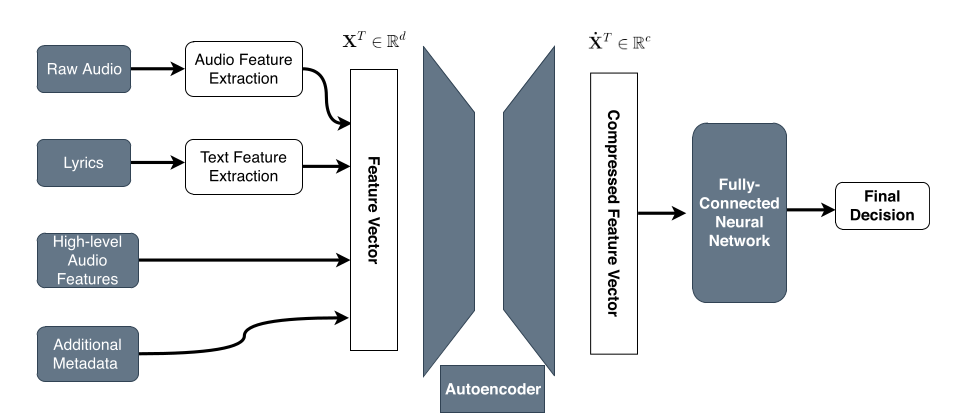
\includegraphics[width=5in]{figs/architecture.png}
    \caption{Model architecture presented by Martin-Gutierrez et al \cite{martin-gutierrez_multimodal_2020}. We intend to replace the fully-connected CNN with an RNN.}
    \label{architecture}
\end{figure}

Li et al \cite{li_lstm-rpa_2021} present LSTM Rolling Prediction Algorithm (LSTM-RPA), a popularity prediction algorithm based on a Recurrent Neural Network. LSTM-RPA breaks the long-term prediction into several short-term trend predictions. This work is an important example of using an RNN architecture to predict song popularity. 
    
Araujo et al \cite{araujo_predicting_2019} present a popularity prediction method using Support Vector Machines; this method predicts whether a song will appear on the Spotify Top 50 Global charts. This work has similar goals to our project and will serve as an important reference for evaluating our model’s accuracy.

In their 2018 paper, Choi et al \cite{choi_comparison_2018} compare audio pre-processing methods for deep neural networks. Their primary result demonstrates that many common preprocessing techniques are redundant; this conclusion will help us inform our pre-processing decisions for our project.

% 
% You need to study the current literature of your planned work. You don't have to exhaust the literature, but you need to search related work with a few proper key words.
% If there are related work, you need to cite them. For example, if you want to cite the ``Deep Learning'' book \cite{goodfellow2016deep}, then you should use the ``\textbackslash cite'' command.
% This section helps you to establish the current status of known knowledge around the project. Particularly, you may consider to cite the research work solving the same problem.  

% \section{Background} ???> Maybe??
% 
% This section is optional. If your project is related to some standard formulations, and you need to introduce details to make your later models clear, you should consider to put these \textbf{standard} formulations here.  For example, if you are going to do some modification of GRU later, but you need to have an introduction of GRU first, then it belongs to this section. A negaive example is, your project will use a GRU layer in a standard way, then a detailed introduction of GRU is not needed. 
% 
% 
% \noindent \textbf{Proposal submission:} When you submit your proposal, you should include the ``Introduction'' and ``Related Work'' sections. If you have a ``Background'' section, you should include it as well. The rubrics for grading your proposal include: 
% \begin{itemize}
% \item 2 points if you have a clear motivation
% \item 3 points if you have a clear summary of your project 
% \item 3 points if you have done at least a rough literature study 
% \item 2 points for the readability of your project (you can use Grammarly to correct your grammar issues.) 
% \end{itemize}
% 
\section{Methods}

\subsection{Dataset}
The data set we used for this experiments was a modified version of the daily top 200 songs by stream count in the Philippines  from January 1st 2017, to May 20th 2021. The problem arose with this Data set when songs would drop off the chart, and potentially come back a few days laters creating "gaps" in our data. In order to somewhat alleviate this problem we filled in large gaps, greater than one or two days with 0 stream counts. Where as smaller gaps were interpolated so that our data is less sparse. The format of the data at this point is tensor of the shape [Timesteps, Stream Count By Song]. The data was still incredibly sparse and in order to further avoid this problem and to form a training and testing set we scanned out data sets for songs which achieved a certain threshold entries over the course of the time. As well to split out data into X values and Y, we took sub-sequences of various sizes, which we referred to as "lookback" with the next time step being the corresponding Y. After trimming our data set in such a manner the shape is 
\[X = [\text{Batch Size, Lookback, Stream Count By Song}]\]
\[Y = [\text{Batch Size, 1, Stream Count By Song}]\]
Due to the sparsity of our data we experimented with different thresholds on whether or not to include a song resulting in a variety of different song sizes. 
As well in order to test our hypothesis one of our architectures has multiple inputs. The second data was formed by obtaining a variety of meta data for each song in the original data set from the spotify API. This meta data includes features such as dancibility or acousticness in the form of a real value from 0 to 1. For each of the songs 13 Meta data features were extracted producing a tensor of shape [Song Count,13]

\subsection{Model Architecture}
The learning problem is a rather basic regression problem. Given the daily stream counts of songs of the course of a certain amount of days, can we accurately predict the stream count of the next day? Given the time oriented nature of the problem the main aspect of our models consisted of recurrent layers.Mostly we experimented with the use of LSTMs as our main layer, but GRUs were also used to a degree of success. We explored both basic models, which consisted of entirely just recurrent layers, and multiple input models which included the previously mentioned meta data. We combined these models such that the output of the recurrent layers were being concatenated to the Meta data and then feed through a basic feed forward network. This architecture turned out to be fruitless, which will be touched on more later, and as such we experienced more success with the basic recurrent models.
% TODO: Better-drawn version of architecture! 

\subsection{Model Evaluation}
Due to being a regression problem we settled on using Mean Squared Error and Root Squared Error as our evaluation metric. As well while not being used as a main metric, in order to visualize the success of our model we plotted the predictions alongside the original amount of stream counts as shown below. \textbf{Graphs here?}


% TODO: output metrics and PLAN for model eval 

% 
% This section should be a detailed introduction of your project. This section should only contain your own work. For example, if you have modified a GRU architecture, this section should only have the modification of GRU. The original GRU structure should be put in the ``Background'' section.  
% 
% In this section, you should have a rigorous introduction of your problem. This list of questions help you to do the formulation,
% \begin{itemize}
% \item What data do you have? How are they denoted ($X$ represents features)? Is every notation well defined (e.g. $X \in \mathcal{R}^d$)? 
% \item What type learning problem it is? What's the desired output from the model? 
% \item What's the input to the model? Is it the same as (part of) the data? Any processing before you can feed the data to the model?
% \item What the model? If the model is not a standard one, do you have a function form of the model?
% \item What's the loss function of the model? If it is not a standard problem, you need to use an equation to show that exactly. 
% \item Can you check all symbols to make sure that every one is well defined?
% \end{itemize}
% 
% 
\section{Experiments}

% TODO: sample graphs 
% TODO: output metrics 
% TODO: comparison between sequential, functional, meta, no meta
% TODO: other model tweaks 

% 
% In this section, you should report your experiments, which that are either related to your hypotheses or the evaluation measures of your models. Do NOT manipulate experiment results, and its OK that the experiment results do not support your hypotheses or expectations. For example, if your project is a modification of the GRU and argues that the motivation can improve its performance. However, the experiment results do not show so. In this section, you should report your observations in experiments. Then you should analyze the results in either of the following ways:
% \begin{itemize}
% \item the original argument is still correct, but experiments are not perfect. There is still a chance that the modification should work.  
% \item the original argument is invalid by observing experiment results. Some part of the argument is wrong. If there is a fix, you can also talk about further modifications.  
% \end{itemize}
% 
\section{Conclusion}
\textbf{Something about sucessful vs unsuccessful models}


While we were unsuccessful in our attempts to use the Meta data of the song to improve performance that may mostly be due to implementation issues. As such it could certainly benefit from further attempts. As well a larger and less sparse data set could be used a most likely would improve performance.
While adding more data would improve the performance it could also lead to complications due to differing music tastes across different regions. By focusing on the Philippines data set  

% TODO: which models were successful and how successful 
% TODO: reiterate the WHY 
% TODO: future work discussion 

% Draw conclusions from this project. Summarize the new findings you want your reader to learn.  
% 
\section{Share of work}
% 
% If the team has more than person, then you should report who has done which part of work. Particularly, you should mention these work items. If multiple people participated in one item, then you can list the percentage of contribution of each person. 
% 
% \begin{itemize}
% \item writing of the proposal 
% \item coding
% \item running experiments and collecting data 
% \item discussions (of project ideas and experiment results) 
% \item writing of the final report 
% \end{itemize}

\bibliographystyle{plain}
\bibliography{sample}

\end{document}
